% -*- TeX:SI -*-
% slovene sub-mode for spell check
\graphicspath{{../}{./}{./slike_UR/}}
%\Large\textbf
\chapter{Manipulacija objektov na tekočem traku \\z robotom Universal Robot UR5e}\label{Pog:UR}

%\vspace{-3.35cm}

%\begin{mdframed}[backgroundcolor=yellow!20, shadow=true,roundcorner=8pt]
%\vspace{-0.35cm}
\section{Cilj vaje}
Pri tej vaji boste uporabljali sodelujočega robota UR5e proizvajalca Universal Robots. Robot ima vgrajen senzor sil in navorov, opremljen pa je z dvoprstnim prijemalom proizvajalca Robotiq. Z robotom boste s tekočega traku pobrali zobnik. Nato boste s pomočjo funkcij, ki jih omogoča sezor sile, z zobnikom poiskali os z zagozdo ter zobnik vstavili na os.
%\end{mdframed}


\section{Universal Robot UR5e}

Robot UR5e danskega proizvajalca Universal Robots spada med sodelujoče robote. Ti roboti so deklarirani kot inherentno varni; kot taki so primerno za delo v skupnem delovnem prostoru s človekom brez dodatnih varnostnih elementov. Robot na podlagi senzorja sile ter ustrezne implementacije dinamičnega modela (primerjave ocenjenih in dejanskih navorov v sklepih) zazna nezaželjene trke z okolico in človekom. V primeru trka robotski krmilnik izvede varnostno nadzorovano ustavitev.

Sodelujoči robot ima 6 prostostnih stopenj, kot je predstavljeno na sliki \ref{fig:ur_conf}. V tabeli \ref{tab:ur_osnovni} so podane nekatere specifikacije manipulatorja.


\begin{figure}[!hbt]
\centering
\includegraphics[width=0.9\textwidth]{ur5e_joints.eps}
\caption{Konfiguracija robota UR5e}
\label{fig:ur_conf}
\end{figure}

\begin{table}
\begin{center}
\caption{Tehnični podatki robota UR5e}
\label{tab:ur_osnovni}
\begin{tabular}{|lr|c|}
\hline Tip &  & UR5e \\
\hline Doseg & & 0.85 m \\
\hline Nosilnost & & 5 kg \\
\hline Maksimalna hitrost vrha & & 1 m/s \\
\hline Ponovljivost & & $\pm 0.03$ mm \\
\hline Delovno območje
     & sklep 1 & $\pm 360^\circ$ \\
     & sklep 2 & $\pm 360^\circ$ \\
     & sklep 3 & $\pm 360^\circ$ \\
     & sklep 4 & $\pm 360^\circ$ \\
     & sklep 5 & $\pm 360^\circ$ \\
     & sklep 6 & $\pm 360^\circ$ \\
\hline Maksimalna hitrost
     & sklep 1 & $180$ $^\circ/s$ \\
     & sklep 2 & $180$ $^\circ/s$ \\
     & sklep 3 & $180$ $^\circ/s$ \\
     & sklep 4 & $180$ $^\circ/s$ \\
     & sklep 5 & $180$ $^\circ/s$ \\
     & sklep 6 & $180$ $^\circ/s$ \\
\hline   Masa &  & $18.4$ kg \\
\hline
\end{tabular}
\end{center}
\end{table}

Robotov uporabniški vmesnik omogoča intuitivno programiranje s široko paleto razširitev za robota (tako strojnih kot programske). Ker je robot intuitiven, fleksibilen ter z majhnim ih odtisom, ga je možno enostavno vključiti v proizvodnji proces neglede na značilnosti objekta ali velikost podjetja.

\section{Online učenje}

Universal Robots omogočajo pridobitev znanja uporabe njihovih robotov preko online izobraževanj. Na njihovi spletni strani je na voljo \emph{Universal Robot Academy}, kjer se spoznate osnovno rokovanje z robotom ter uporabo nekaterih funkcij. Akademija je na voljo na naslovu https://www.universal-robots.com/academy/ (izberete program za \emph{e-Series}).  \textbf{Priporočamo, da pred vajo opravite online trening.}


\section{Ročna učna naprava}

Programiranje robota poteka preko ročne učne naprave, na kateri je nameščeno programsko okolje PolyScope (slika \ref{fig:ur_tp}). Ročna učna naprava omogoča upravljanje z robotsko roko in krmilnikom ter pisanje, urejanje in poganjanje programov.


\begin{figure}[!hbt]
\centering
\includegraphics[width=0.6\textwidth]{ur5e_tp.eps}
\caption{Ročna učna naprava}
\label{fig:ur_tp}
\end{figure}

Elementi ročne učne naprave, predstavljene na sliki \ref{fig:ur_tp}, so:
\begin{enumerate}
  \item gumb za ustavitev v sili,
  \item gumb za prižig robota,
  \item gumb za omogočanje vodenja z roko,
  \item glavni meni,
  \item gumbi za izvajanje programa,
  \item orodna vrstica z zavihki za interaktivne menije,
  \item status robota,
  \item urejevalnik programa in nastavitev.
\end{enumerate}

\subsection{Zagon krmilnika in robotske roke}
\label{ch:zagon}

Krmilnik vsebuje fizične električne vhodno/izhodne povezave, ki povezujejo robotsko roko, ročno učno napravo in ostalo periferijo. Za vodenje robotske roke morate zagnati krmilnik.

\begin{itemize}
  \item Na \textbf{ročni učni napravi} pritisnite gumb za zagon.
  \item  Počakajte, da se na zaslonu prikažejo besedilo nameščenega operacijskega sistema in
gumbi programa.
  \item  Ko se pojavi okno \emph{Cannot Proceed} izberite \textbf{Go to initialization screen} za dostop do zaslona \emph{Initialize}.
\end{itemize}

Barvni indikator v spodnjem levem kotu zaslona nakazuje stanje robota:
\begin{itemize}
\item rdeča -- robotska roka je ustavljena.
\item rumena -- robotska roka je vključena, a ni pripravljena za normalno delovanje.
\item zelena -- robotska roka je vključena in pripravljena za normalno delovanje.
\end{itemize}

Za zagon robota:
\begin{itemize}
    \item Izberite gumb \textbf{ON} z zeleno LED za zagon inicializacijskega procesa. Lučka LED se nato spremeni v rumeno, s čimer nakaže, da je robot vključen in v stanju pripravljenosti.
    \item Izberite gumb \textbf{START}, da sprostite zavore.
    \item Izberite gumbe \textbf{OFF} z rdečo LED za izklop robotske roke.
\end{itemize}



\section{Zavihek Move}

Na zavihku \emph{Move} se nahajajo gumbi za premikanje robota. Robota lahko tu premikate po posameznih sklepih ali pa spreminjate lego vrha robota. Srednje okno predstavlja vizualizacijo trenutne lege robota. Pri tem sta označena bazni koordinatni sistem in koordinatni sistem vrha, sam vrh robota (TCP -- \emph{tool center point}) pa je označen z modro kroglo.

\begin{figure}[!hbt]
\centering
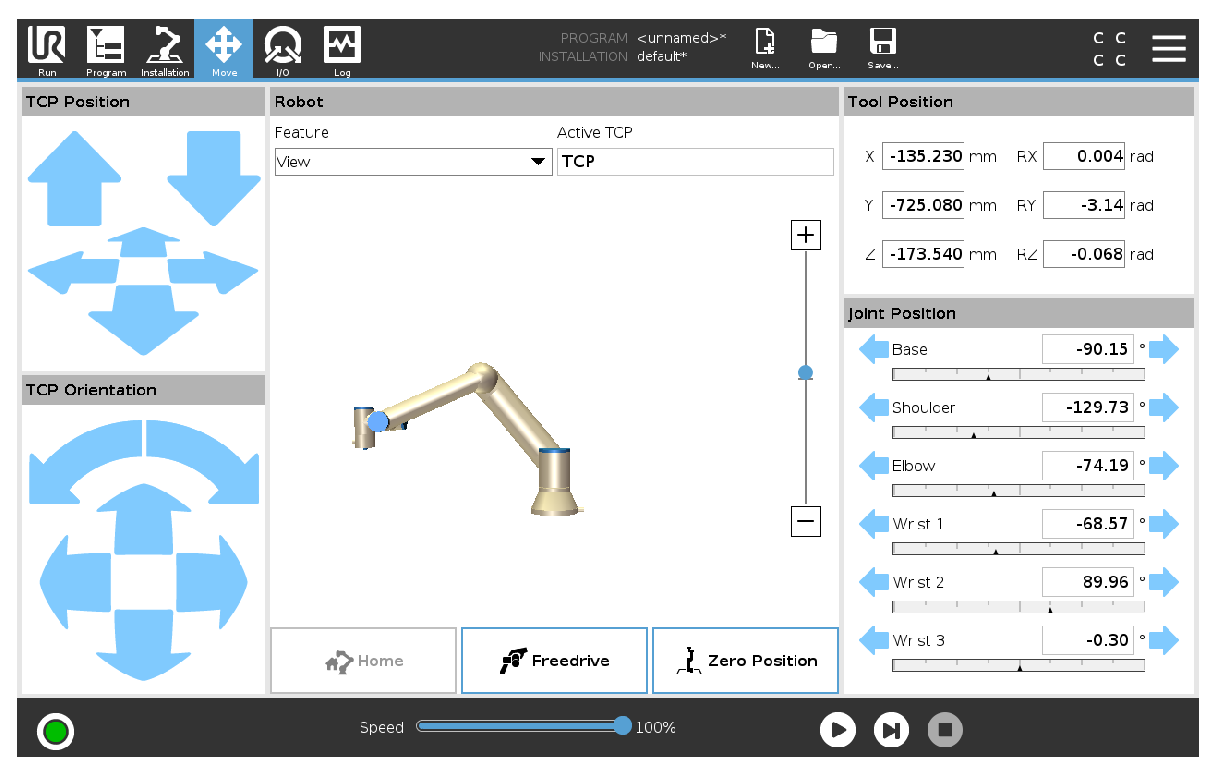
\includegraphics[width=0.7\textwidth]{ur5e_tab2.eps}
\caption{Zavihek Move v okolju PolyScope}
\label{fig:ur_tab2}
\end{figure}

Za premikanje robota v ustrezni smeri držite pritisnjeno ustrezno puščico na zaslonu. S puščicami pri \emph{TCP Position} spreminjate položaj vrha robota, s puščicami pri \emph{TCP Orientation} pa orientacijo vrha robota. Točka vrtenja je določena z \emph{Active TCP}.

V predelku (\emph{Joint Position}) lahko premikate posamezen sklep. Pri tem upoštevajte, da ima vsak sklep omejitev $\pm 180^\circ$

če pritisnite in držite gumb \emph{Freedrive}, omogočite premikanje robota z roko -- enaka funkcionalnost, kot če držite gumb na vrhnji strani ročne učne enote.

\section{Zavihek Program}

Robotski ukazi so združeni v programskem drevesu. Za ustvarjanje novega programa sledite spodnjemu postopku.

\begin{enumerate}
\item V urejevalniku programov in nastavitev (sredina zgornje vrstice)  izberite \textbf{New...} in \textbf{Program}.
\item V urejevalniku programov in nastavitev izberite \textbf{Save...} in \textbf{Save All}.
\item V \emph{File Path} preverite, če je izpisano ime novega programa.
\end{enumerate}

Na levi strani zavihka \emph{Program} je seznam štirih skupih ukazov:
 \begin{itemize}
   \item Osnovni (\emph{Basic})  -- seznam osnovnih ukazov za premikanje, I/O, pavza, ipd.;
   \item Napredni (\emph{Advanced}) -- seznam naprednih ukazov;
   \item Predloge (\emph{Templates}) -- predloge za različne funkcionalnosti robota (npr. paleta, vodenje po sili, tekoči trak);
   \item \emph{URCaps} -- funkcionalnosti dodatne opreme (npr. prijemala, kamera, senzor sil in navorov).
 \end{itemize}

\begin{figure}[!hbt]
\centering
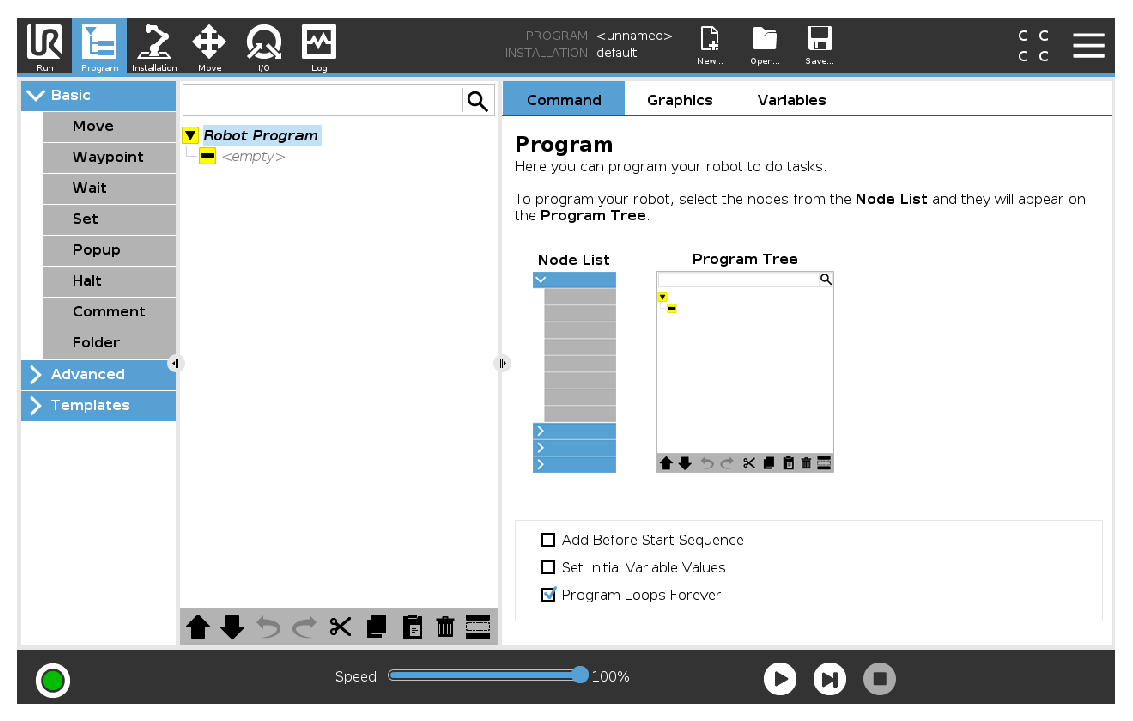
\includegraphics[width=0.7\textwidth]{ur5e_tab1.eps}
\caption{Zavihek \emph{Program} v okolju PolyScope}
\label{fig:ur_tab1}
\end{figure}

Vsak ukaz ima v osnovi tri možne zavihke na desni polovici ekrana, ki nadzorujejo splošno obnašanje programa. Zavihek \textbf{Command} vsebuje splošne nastavitve posameznega ukaza. če izbere programsko vozlišče \emph{Robot Program}, dobite na voljo tri izbire:
\begin{itemize}
  \item \textbf{Add Before Start Sequence} -- ta opcija omogoča izvedbo kode pred zagonom robotskega programa (npr. inicializacija spremenljivk, prijemal).
  \item \textbf{Set Initial Variables Values} -- tu se nastavijo začetne vrednosti spremenljivk.
  \item \textbf{Program Loops Forever} -- ta opcija omogoča izvajanje robotskega programa v neskončni zanki (v nasprotnem primeru se program izvede samo enkrat).
\end{itemize}

V zavihku \textbf{Graphics} je grafično predstavljena trenutna konfiguracija robota. Pot TCP je prikazana v 3D pogledu, kjer zelene točke predstavljalo posamezne naučene točke (\emph{Waypoints}). Senca robota nakazuje lego robota v trenutno izbrani točki v robotskem programu.

V zavihku \textbf{Variables}  je seznam aktivnih spremenljivk robotskega programa in njihovih vrednosti. Pokaže se samo v primeru, da je kakšna spremenljivka aktivna. če želite prikazovati vrednosti točk, morate izbrati opcijo \emph{Show Waypoints}.


\subsection{Programski ukazi}

Tipični programski ukazi so predstavljeni v nadaljevanju.

\begin{figure}[!hbt]
\centering
\includegraphics[width=\textwidth]{ur5e_tab4.eps}
\caption{Programski ukazi: Move, Waypoint, Wait,  Set}
\label{fig:ur_tab3}
\end{figure}

%%%%
%%%%
%%%% DODAJ NOVE SLIKE!!!!!!!!!!!!
%%%%
%%%%
% move
% waypoint
% wait
% loop
% assigment
% if
% script


\subsubsection{Move}

Ukaz \emph{Move} opisuje gibanje robota med osnovnimi smernimi točkami (\emph{Waypoints}). Smerne točke morajo biti vgnezdene pod ukazom \emph{Move}. Z ukazom \emph{Move} definirate hitrost in pospešek gibanja robota med posameznimi točkami.

Na voljo so trije tipi gibanja:
\begin{itemize}
  \item \emph{\textbf{moveJ}} je gibanje definirano v sklepnem prostoru robota. Gibanje sklepov je sinhrono; gibanje vseh sklepov se začne in konča istočasno (posledično se sklepi gibljejo z različnimi hitrostmi). V primeru uporabe giba \emph{MoveJ} se definira gibanje sklepov, gibanje vrha robota pa ni definirano. Pri tem tipu giba se defiranjo hitrosti in pospeški sklepov (deg/s in deg/s${}^2$). Gib se uporablja takrat, ko je zaželeno hitro gibanje robota, pri čemer nedefinirano gibanje vrha ni problematično; pri prehodih med točkami z velikimi razlikami v sklepih; pri prehodih čez singularne lege.
  \item \emph{\textbf{moveL}} je linearni premik vrha robota (TCP) med posameznimi točkami, kar posledično pomeni bolj kompleksno gibanje posameznih sklepov za zagotavljanje linearnosti giba. Gibu se lahko predpišeta hitrost in pospešek (mm/s in mm/s${}^2$).
  \item \emph{\textbf{moveP}} je premik s konstantno hitrostjo in definiranim radijem. Uporablja se ga pri aplikacijah kot so lepljenje ali nanašanje materiala. Radij kroženja je privzet pri vseh točkah v tem gibu. Manjša vrednost radija rezultira v ostrejših gibih, medtem ko se večji radiji kažejo v bolj gladkih gibih.
\end{itemize}

\subsubsection{Waypoint}

Naučena lega robota je shranjena v \emph{Waypoint}, in predstavlja robotu referenco, kam naj se premakne. Točke se nauči s fizičnim premikanjem robota v ustrezno lego.

\emph{Waypoint} opisuje relacijo med trenutno izbranim vrhom robota (TCP) in trenutno aktivnim koordinatnim sistemom (bazni ali pa uporabniški koordinatni sistem). \emph{Waypoint} vedno nastopa v kombinaciji z ukazom \emph{Move}. Pod en \emph{Move} je lahko ugnezdenih več točk.

Točke se lahko kopira (orodja v spodnji vrstici pod programskim drevesom) ali pa se uporabi gumb \emph{Link} v zavihku \emph{Command}.


\subsubsection{Wait}

Ukaz \emph{Wait} začasno ustavi oz. zakasni vhodno/izhodni signal ali izraz za ustrezno število sekund. Ostale možnosti vključujejo še čakanje na ustrezen digitalni oziroma analogni signal.


\subsubsection{Set}

Ukaz \emph{Set} postavi digitalni oziroma analogni izhod na dano vrednost. Digitalni izhod se lahko uporabi tudi kot samo pulz.

Z ukazom \emph{Set} lahko programsko spreminjamo nastavljeno obremenitev robota.


%\subsection{Loop}
%
%Ukaz \emph{Loop} (meni \textbf{Advanced} na levi strani) ponavlja vgnezdene osnovne ukaze programa. Osnovni ukazi programa se lahko ponavljajo v neskončnost (\emph{Loop always}), določeno število (\emph{Loop X times}) ali dokler je določen pogoj resničen. Ko se ukaz ponovi določeno število krat, se ustvari dodeljena spremenljivka zank (imenovana \verb"Loop_1"), ki se lahko uporablja v izrazih znotraj zanke. Spremenljivka zanke šteje od $0$ do $N-1$.
%
%\subsubsection{Assignment}
%
%Ukaz \emph{Assignment} priredi spremenljivki na levi strani ustrezno vrednost, določeno z izrazom na desni strani.
%
%\begin{mdframed}[backgroundcolor=yellow!10, shadow=true,roundcorner=8pt]
%\textbf{Primer:} če želite definirati točko \verb"tocka_nad", ki je postavljena 30~mm nad točko \verb"tocka0", uporabite funkcijo \verb"pose_add" kot je prikazani na primeru.
%\begin{verbatim}
%tocka_nad = pose_add(tocka0, p[0,0,0.03,0,0,0])
%\end{verbatim}
%\end{mdframed}
%Deklaracija \verb"p[x,y,z,ax,ay,az]" definira vektor lege s tremi translacijami (\verb"x", \verb"y", \verb"z") in tremi rotacijami (\verb"ax", \verb"ay", \verb"az"). Funkcija  \verb"pose_add" definira novo točko, ki je od izvorne točke premaknjena za ustrezen premik \verb"p[]" v globalnem koordinatnem sistemu.
%
%
%\subsubsection{If}
%
%Pogojni stavek strukture \textbf{If...Else} spremeni delovanje robota glede na senzorno informacijo ali pa vrednost spremenljivke. Z ustrezno strukturo izraza \emph{f(x)} se definira pogoj; v primeru da je pogoj izpolnjen (\verb"True"), se izvede koda znotraj ukaza \emph{If}.
%
%Ukaz \emph{If} je lahko sestavljen iz več pogojnih stavkov \emph{ElseIf} -- doda se jih z izbiro možnosti \emph{Add ElseIf}, odstrani pa z izbiro \emph{Remove ElseIf}. \emph{If} stavek lahko vsebuje samo en \emph{Else}.
%
%\begin{mdframed}[backgroundcolor=blue!20, shadow=true,roundcorner=8pt]
%Izberete lahko možnost \textbf{Check expression continuously}, ki omogoča sprotno preverjanje pogoja med izvajanjem vgnezdenega programa. če pogoj ni več izpolnjen (pogoj je \verb"False"), potem se izvede ustrezen \emph{Else} oziroma \emph{ElseIf}.
%\end{mdframed}
%
%
%\subsubsection{Script}
%
%Ukaz \emph{Script} se lahko uporablja kot vrstico ukaza (podobno kot \emph{Assignment}) ali kot datoteka, kjer lahko urejate URScrip kodo.
%
%Ustrezni ukazai in struktro URScript kode se nahaj v \emph{Script Manual} na strani proizvajalca robota pod zavihkom \emph{Support} (http://www.universal-robots.com/support).
%
%Funkcije in spremenljivke, deklarirane v URScript datoteki, so na voljo skozi celotno izvajanje programa v okolju PolyScope.
%
%\begin{mdframed}[backgroundcolor=yellow!10, shadow=true,roundcorner=8pt]
%\textbf{Primer:} če želite spremeniti samo komponento \verb"z" v naprej definirane točke \verb"tocka_1", lahko uporabite ukaz \emph{Assignment} in ustrezen ukaz \verb"pose_add",  ali pa preprosto spremenite samo ustrezno komponento naučene točke z uporabo ukaza \emph{Script}.
%\begin{verbatim}
%tocka_1[2] = tocka_1[2]+0.03
%\end{verbatim}
%\end{mdframed}
%Številka v oglatih oklepajih \verb"[]" definira komponento vektorja točke; številka \verb"2" nakazuje, da je to pozicija v smeri  z.
%


%\subsubsection{Script}
%
%The following options are available in the drop down list under Command:
%\begin{itemize}
%  \item \textbf{Line} allows you to write a single line of URscript code, using the Expression Editor
%  \item \textbf{File} allows you to write, edit or load URscript files.
%\end{itemize}
%
%You can find instructions for writing URscript in the Script Manual on the support website (http://www.universal-robots.com/support).
%
%Functions and variables declared in a URscript file are available for use througout the program in the PolyScope.

%\subsubsection{Pallet}
%
%A pallet operation can perform a sequence of motions in a set of places given as a pattern. At each of the positions in the pattern, the sequence of motions will be run relative
%to the pattern position.
%
%Programming a Pallet Operation requires the following steps:
%\begin{itemize}
%  \item Define the pattern.
%  \item Make a PalletSequence for picking up/placing at each single point. The sequence describes
%what should be done at each pattern position.
%  \item Use the selector on the sequence command screen to define which of the waypoints in the
%sequence should correspond to the pattern positions.
%\end{itemize}
%
%In a \textbf{Pallet Sequence} node, the motions of the robot arm are relative to the pallet position. The
%behavior of a sequence is such that the robot arm will be at the position specified by the pattern
%at the Anchor Position/Pattern Point. The remaining positions will all be moved to make this fit.
%Do not use the Move command inside a sequence, as it will not be relative to the anchor position.
%
%\begin{figure}[!hbt]
%\centering
% \includegraphics[width=0.7 \textwidth]{ur5e_tab5.eps}
%\caption{Pallet definition}
%\label{fig:ur_tab5}
%\end{figure}
%
%
%The \textbf{Pattern} command can be used to cycle through positions in the robot program. The Pattern
%command corresponds to one position at each execution.
%A pattern can be given as one of four types. The first three, \textbf{Line}, \textbf{Square} or \textbf{Box} can be used
%for positions in a regular pattern. The regular patterns are defined by a number of characteristic
%points, where the points define the edges of the pattern. For Line this is the two end points, for
%Square this is three of the four corner points, where as for Box this is four of the eight corner
%points. The programmer enters the number of positions along each of the edges of the pattern.
%The robot controller then calculates the individual pattern positions by proportionally adding the
%edge vectors together.
%
%A counter variable is used while traversing the positions of the pattern. The name of the variable
%can be seen on the Pattern command screen. The variable cycles through the numbers from 0
%to the number of points in the pattern $-1$. This variable can be manipulated using
%assignments, and can be used in expressions.

\section{Zavihek Installation}

V zavihku  \emph{Installation} se nahajajo možnosti za nastavljanje parametrov orodja (TCP), nastavitev funkcionalnosti kot so tekoči trak, vijačenje, varnostnih parametrov, globalno definiranih točk, premic, ravnin (\emph{Features}), komunikacije in vtičnikov \emph{URCaps}. Vse te nastavitve se shranijo v datoteko \emph{Installation}, ki je vidna na sredini zgornje vrstice.

\subsection{Nastavitev orodja}

Središčna točka orodja (\emph{Tool Center Point} -- TCP)  je točka na vrhu robotskega prijemala. Povezuje relativni premik iz vrh robotskega manipulatorja v TCP orodja. Pomembno je, da je TCP ustrezno nastavljen, saj se naučene točke robota shranijo kot relacija TCP glede na ustrezen koordinatni sistem (bazni, uporabniški). če je TCP napačen, se robot pri izvajanju ne postavi v naučeno točko.

V meniju \emph{General > TCP} nastavite lego orodja (\emph{Position} in \emph{Orientation}). Pri tem lahko ustrezne podatke vpišete ročno (\emph{X, Y, Z, RX, RY, RZ}) ali pa uporabite čarovnika (klik na ikono s čarobno palico, nato pa sledite interaktivnim navodilom). Nastavi se tudi ustrezno obremenitev (\emph{Payload}) in težišče orodja (\emph{CX,CY,CZ}). Zavedati se morate, da je za pravilno delovanje varnostnih funkcij potrebno spreminjati nastavljeno obremenitev med samim izvajanjem programa. S tem se zagotovi pravilen preračun obremenitev robota na podlagi dinamičnega modela, ki vključuje tudi maso prijetega objekta.



\subsection{Koordinatni sistemi -- Features}

Meni \emph{Features} združuje uporabniško določene koordinatne sisteme, ki se jih definira na podlagi osnovnih geometrijskih elementov: točko, premico in ravnino. Uporabniške koordinatne sisteme se lahko pripiše posameznemu objektu, ki ga aplikacija obravnava in ni del robotske roke: miza, drugi stroji, obdelovanci, tekoči trak, paleta, navidezne meje.

Vedno sta definirana dva elementa, ki imata legi definirani glede na robotsko roko:
\begin{itemize}
  \item \emph{Base} -- baza je postavljena v izhodišče globalnega/baznega koordinatnega sistema,
  \item \emph{Tool} -- orodje se nahaja v izhodišču trenutnega TCP.
\end{itemize}


\begin{figure}[!hbt]
\centering
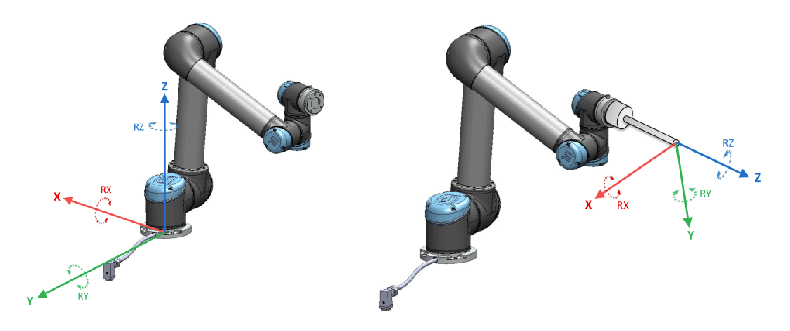
\includegraphics[width=0.7\textwidth]{ur5e_feat.eps}
\caption{Koordinatna sistema baze in orodja}
\label{fig:ur_feat}
\end{figure}

Uporabniški koordinatni sistemi so določeni v delovnem prostoru robota glede na trenutno lego izbranega TCP. Nauči se jih preko vodenja z roko (\emph{Freedrive}) ali klasičnega premikanja po oseh. Koordinatni sistem se lahko nauči na tri načine:
\begin{itemize}
    \item \emph{Point} -- točka določa položaj izhodišča koordinatnega sistema, orientacija pa sovpada z orientacijo izbranega TCP;
    \item \emph{Line} -- z izbiro premice se definira linijo, ki ji robot lahko sledi (npr. pri tekočem traku); linija je definirana kot povezava med dvema naučenima točkama (smer y), smer z je definirana kot projekcija osi z prve točke na ravnino, kateri normala je os y, izhodišče linije pa predstavlja prva naučena točka;
    \item \emph{Plane} -- ravnina je definirana s tremi točkami; prva točka predstavlja izhodišče, druga točka pozitivno os x, tretja točka pa pozitivno os y, os z pa je določena v smislu desnosučnega koordinatnega sistema.
\end{itemize}



\section{Zagon programa}

Za zagon programa kliknete na gumb  \textbf{Play} na sredini spodnje vrstice uporabniškega vmesnika.

če robot pred zagonom programa ni v začetni legi, se pojavi okno \emph{Move Robot into Position}. Okno se pojavi tudi v primeru, ko se robot premika proti željeni točki med spreminjanjem programa. če se robot ne more premakniti do začetne točke, se premakne do prve dosegljive točke v programu.

Za premik robota v začetno lego držite tipko \emph{Auto}.


\section{Prijemalo Robotiq Hand-E}

Robotsko prijemalo Robotiq Hand-E ima dva prsta z nastavljivim hodom, hitrostjo in silo prijemanja. Zaradi svoje univerzalne zasnove lahko izvede prijemanje po sili  (notranje ali zunanje prijemanje) ali pa prijemanje po obliki. Nosilnost prijemala je 5~kg, pozicijska ponovljivost pa je 0,05~mm. Na sliki \ref{fig:ur_gripper} so predstavljene dimenzije prijemala.

\begin{figure}[!hbt]
\centering
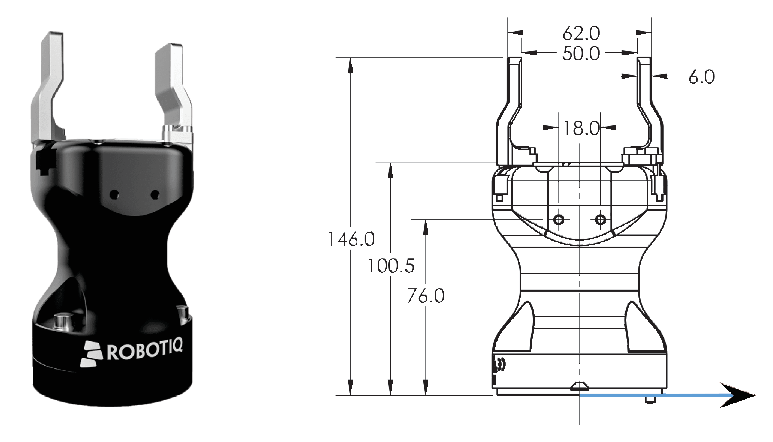
\includegraphics[width=0.7\textwidth]{ur5e_gripper.eps}
\caption{Robotsko prijemalo \emph{Robotiq Hand-E}}
\label{fig:ur_gripper}
\end{figure}

\subsection{Aktivacija prijemala}

Pred uporabo prijemala je le-tega potrebno  aktivirati; v nasprotnem primeru se na ekranu pojavi opozorilo. Aktivacijo se lahko izvede ročno z \textbf{Installation > URCaps > Gripper > Dashboard > Scan > Activate}.  Prijemalo mora biti aktivirano ob vsakem ponovnem zagonu programa, zato je priporočljivo, da se v program doda kodo za avtomatsko aktivacijo prijemala. Kodo se doda v sekcijo \textbf{BeforeStart} na sledeči način
\begin{itemize}
    \item v \textbf{Program > Basic Command} izberite \textbf{Add Before Start Sequence}
    \item v sekcijo \emph{Before Start} vstavite \textbf{Program > URCaps > Gripper Activator > Activate}.
\end{itemize}

\subsection{Uporaba prijemala}

Za odpiranje in zapiranje prijemala uporabite ukaza \textbf{Gripper open} in \textbf{Gripper close}, ki sta na voljo preko menija \textbf{Program > URCaps > Gripper > Edit action > Open/Close > Save action}. Prijemalo se lahko premakne tudi ročno preko ikone \textbf{UR+} ter nato menija prijemala v zgornjem desnem kotu uporabniškega vmesnika.

S funkcijo \textbf{Edit action} nastavite hitrost in silo prijemanja. Hitrost se lahko nastavi med 20~mm/s in 150~mm/s, silo prijemanja pa med 20~N in 235~N.

\begin{figure}[!hbt]
\centering
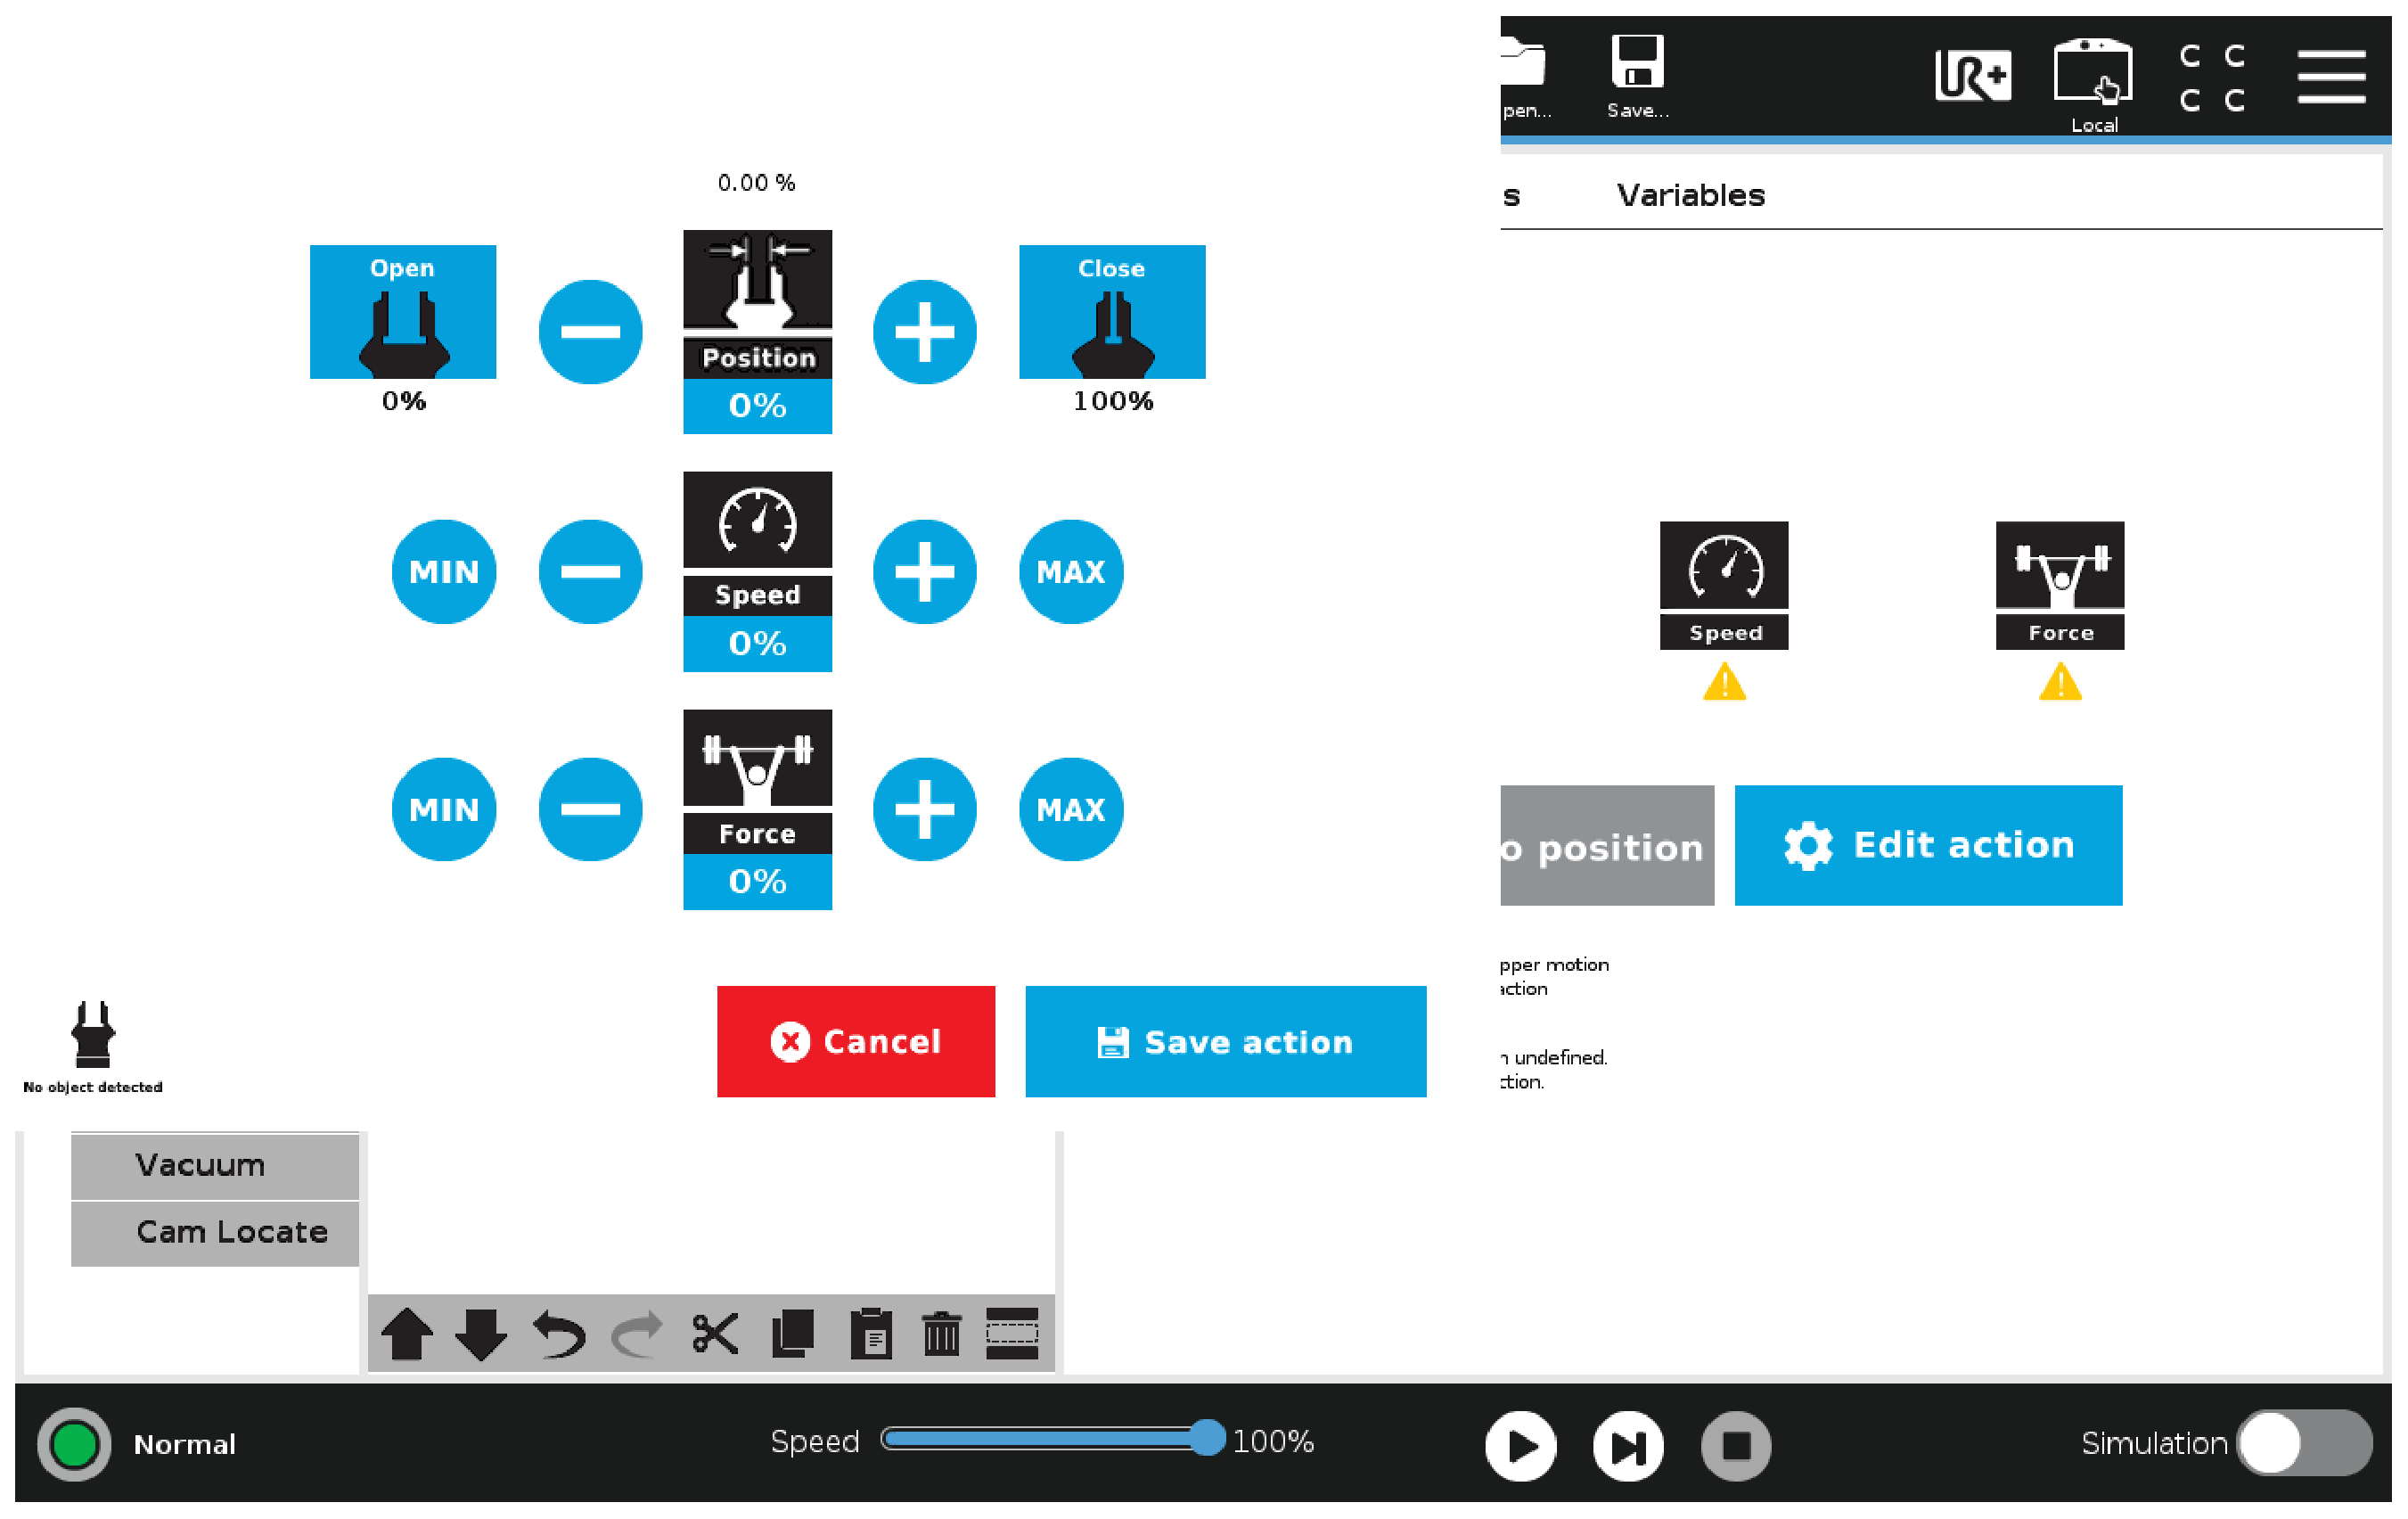
\includegraphics[width=0.7\textwidth]{ur5e_urcap_grip.eps}
\caption{Nastavljanje giba in parametrov prijemala}
\label{fig:ur_gripper1}
\end{figure}


\section{Senzor sil in navorov}

Robotska roka je opremljena z integriranim 6D senzorjem sil in navorov na vrhu robota. Območje merjenja sile je 50~N (resolucija 2,5~N, natančnost 4,0~N), območje merjenja navora pa 10~Nm (resolucija 0,04~Nm, natančnost 0,30~Nm).

Najbolju pogosto uporabljena ukaza za uporabo senzorja sil in navorov sta
\begin{itemize}
  \item \verb"zero_ftsensor()" -- ta funkcija ponastavi neobremenjen senzor; vključena mora biti v sekvenco \emph{Before Start};
  \item \verb"force()" -- funkcija vrne rezultanto zunanjih sil, ki delujejo na TCP (vrnjena sila se izračuna kot aritmetična sredina sil Fx, Fy, in Fz, dobljenih z ukazom \verb"get_tcp_force()").
\end{itemize}

\newpage

\subsection{Ukaz \emph{Insertion}}

Senzor sile se  uporablja za premikanje robota z roko pri učenju, seveda pa ima dodano vrednost tudi pri izvajanju aplikacij, kjer je potreben kontakt robota z obdelovancem in okolico (na primer, vstavljanje kosa v primež, vijačenje, brušenje).

Ukaz \emph{URCaps > Insertion} ima na voljo tri načine interakcije (slika \ref{fig:ur_insertion})
\begin{itemize}
  \item spiralno gibanje: ob kontaktu se robot giblje po spirali, da najde poti z najmanjšim uporom (npr. vstavljanje čepa v luknjo);
  \item rotacijsko gibanje: ob kontaktu robot rotira objekt, dokler ne najde poti z najmanjšim uporom (npr. sinhroniziranje zobnikov);
  \item linearno gibanje: gibanje sledi spriralnemi oz. rotacijskemu gibanju, robot se linearno premika v izbrani smeri, dokler ne zazna predpisane sile.
\end{itemize}
Omenjeni načini interakcije so namenjeni uporabi pri vstavljanju objektov v luknje oziroma izvrtine ter pri kontaktih s površino.

\begin{figure}[!hbt]
\centering
\includegraphics[width=0.6\textwidth]{ur5e_insertion.eps}
\caption{Trije načini interakcije: 1) spirala, 2) rotacija in 3) linearni premik}
\label{fig:ur_insertion}
\end{figure}


\subsubsection{\emph{Spiral}}

Nastavitve spiralnega giba so predstavljene na sliki \ref{fig:ur_spir}.
\begin{figure}[!hbt]
\centering
\includegraphics[width=0.6\textwidth]{ur5e_spiral.eps}
\caption{Nastavitve spiralnega giba}
\label{fig:ur_spir}
\end{figure}

\begin{enumerate}
  \item \emph{Teach positon} -- shrani lego objekta kot ciljno točko; pomembna je samo koordinata z;
  \item \emph{Reference frame} -- koordinatni sistem, glede na katerega se bo premikalo orodje;
  \item \emph{Axis} -- os, vzdož katere se bo premikalo orodje;
  \item \emph{Advanced parameters} -- dodatne nastavitve;
  \item \emph{Speed} -- hitrost gibanja v mm/s;
  \item \emph{Force initiating spiral move} -- sila, ki jo mora izmeriti senzor ob kontaktu, da se inicializira spiralno gibanje;
  \item \emph{Force initiating insertion} -- sprememba sile, ki je potrebna, da robot zazna pot z najmanjšim uporom;
  \item \emph{Radius increment per turn} -- za koliko se poveča radij spirale na obrat;
  \item \emph{Enable peck mode} -- vklop odmikanja orodja med kontakti;
  \item \emph{Maximum radius} -- največji možen radij spirale.
\end{enumerate}

\subsubsection{\emph{Rotational}}

Nastavitve rotacijskega giba so predstavljene na sliki \ref{fig:ur_rotat}.
\begin{figure}[!hbt]
\centering
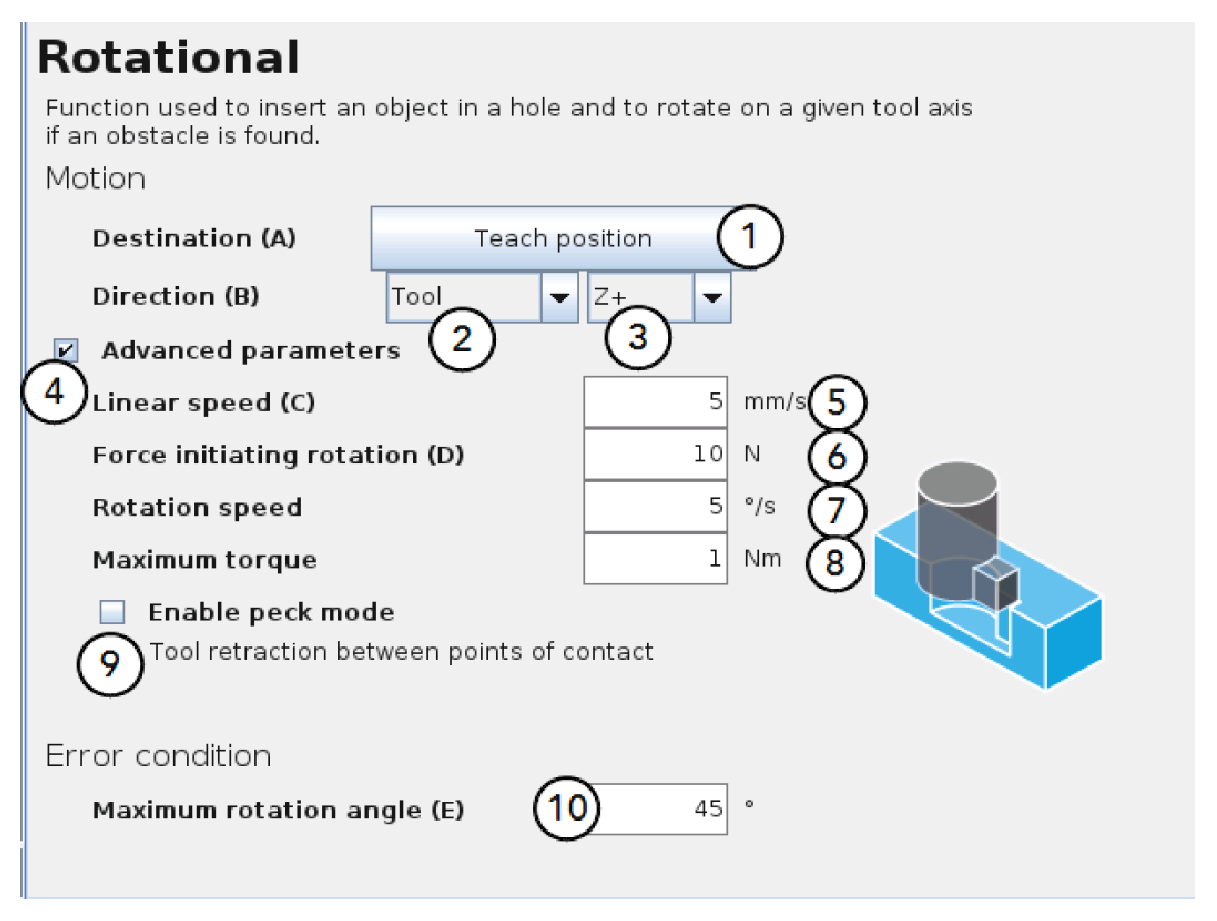
\includegraphics[width=0.6\textwidth]{ur5e_rotational.eps}
\caption{Nastavitve rotacijskega giba}
\label{fig:ur_rotat}
\end{figure}

\begin{enumerate}
  \item \emph{Teach positon} -- shrani lego objekta kot ciljno točko; pomembna je samo koordinata z;
  \item \emph{Reference frame} -- koordinatni sistem, glede na katerega se bo premikalo orodje;
  \item \emph{Axis} -- os, vzdož katere se bo premikalo orodje;
  \item \emph{Advanced parameters} -- dodatne nastavitve;
  \item \emph{Linear speed} -- hitrost premikanja robota proti ciljni točki;
  \item \emph{Force initiating rotation} -- sila, ki jo mora izmeriti senzor ob kontaktu, da se inicializira rotacijsko gibanje;
  \item \emph{Rotation speed} -- hitrost vrtenja robota v ${}^\circ$/s;
  \item \emph{Maximum torque} -- največji dovoljen navor;
  \item \emph{Enable peck mode} -- vklop odmikanja orodja med kontakti;
  \item \emph{Maximum rotation angle} -- največji možen kot rotacije.
\end{enumerate}


\subsubsection{\emph{Linear}}

Nastavitve translacijskega giba so predstavljene na sliki \ref{fig:ur_linear}.
\begin{figure}[!hbt]
\centering
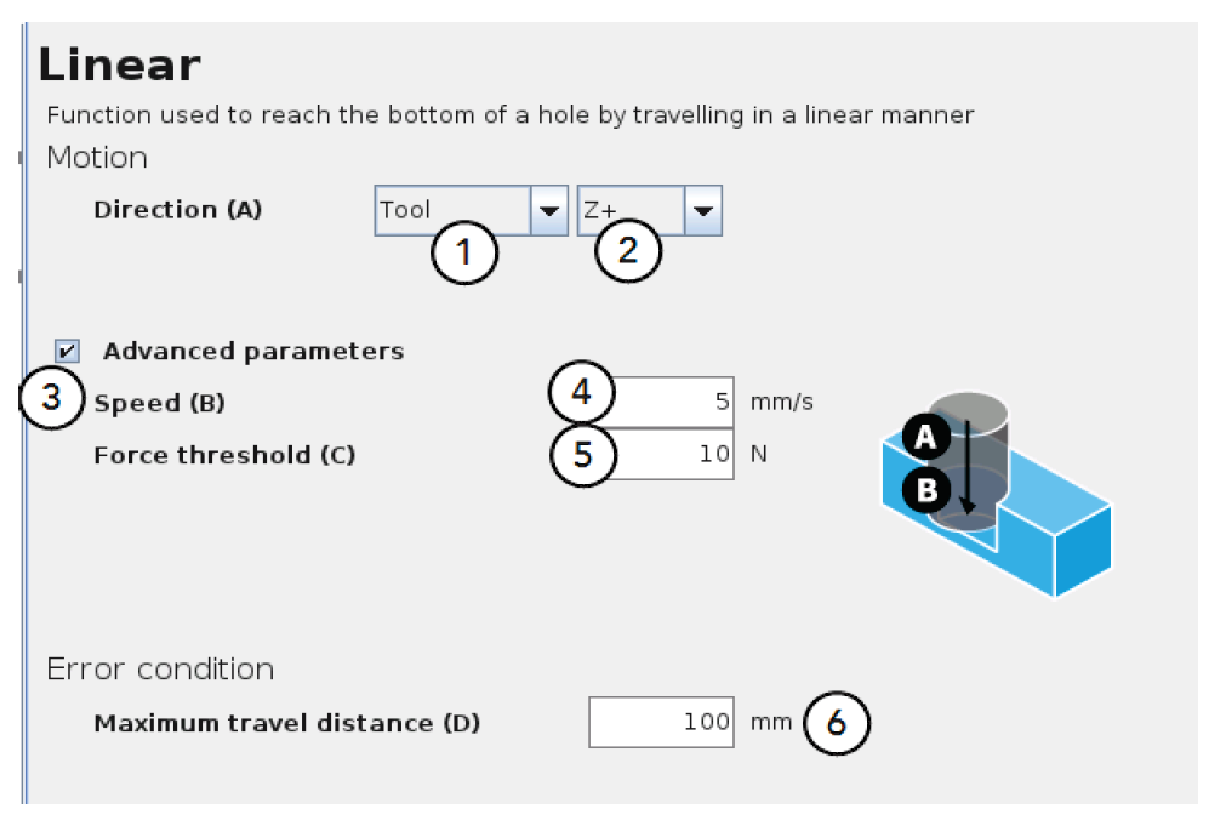
\includegraphics[width=0.6\textwidth]{ur5e_linear.eps}
\caption{Nastavitve linearnega giba}
\label{fig:ur_linear}
\end{figure}

\begin{enumerate}
  \item \emph{Reference frame} -- koordinatni sistem, glede na katerega se bo premikalo orodje;
  \item \emph{Axis} -- os, vzdož katere se bo premikalo orodje;
  \item \emph{Advanced parameters} -- dodatne nastavitve;
  \item \emph{Speed} -- hitrost premikanja robota proti ciljni točki;
  \item \emph{Force threshold} -- sila, ki jo mora izmeriti senzor, da robot zaključi z gibanjem;
  \item \emph{Maximum travel distance} -- največja razdalja, ki jo robot lahko prepotuje.
\end{enumerate}

%\section{Zapestna kamera Robotiq}
%
%Kamera, nameščena v zapestje robota, ima barvni CMOS senzor z nastavljivo resolucijo od 0,3 to 5~Mpx, frekvenco osveževanje od 2 do 30 FPS in avtomastko ostrenje slike od 70~mm do neskočnosti. Kamero se uporablja za prepoznavo in lokalizacijo objektov, programska oprema pa omogoča prepoznavo večih objektov.
%
%Pred uporabo je potrebno izvesti kalibracijo kamere, kar se stori z uporabo kalibracijske plošče s šahovnico z znano velikostjo polj. Kalibracija je vezana na dotično lego kamere, imenovano \emph{Snapshot Position}. Postopek kalibracije kamere je prikazan na sliki \ref{fig:ur_snapshot}.
%
%\begin{figure}[!hbt]
%\centering
% 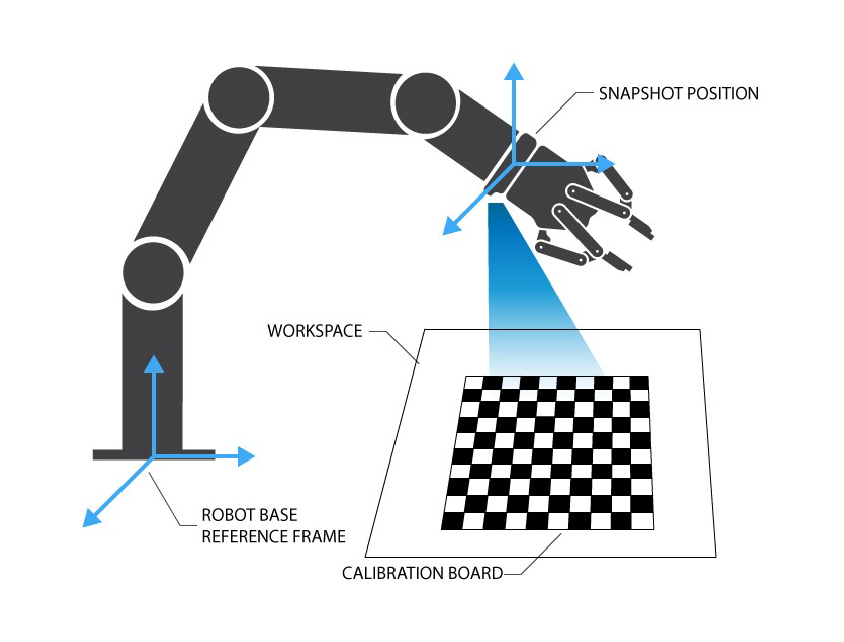
\includegraphics[width=0.6\textwidth]{ur5e_snapshot.eps}
%\caption{Shematični prikaz kalibracije kamere in uporabe \emph{Snapshot position}}
%\label{fig:ur_snapshot}
%\end{figure}
%
%Kalibracija kamere s pripadajočo lego kamere je že v naprej pripravljena - naložite jo z izbiro ustrezne \emph{Install} datoteke.
%
%\subsection{Prepoznava objekta}
%
%Ko naložite ustrezno \emph{Install} datoteko, lahko z uporabo ukaza \emph{Camera Locate} znotraj UR programa naučite prepoznova iskanega objekta. Z enim ukazom \emph{Camera Locate} lahko naučite samo en tip objekta, obenem pa lahko prepoznate več istih objektov. če aplikacija zahteva prepoznavo več različnih objektov, potem je potrebno uporabiti ustrezno število ukazov \emph{Camera Locate}. Prepoznava objekta je vezana na \emph{Snapshot position}; če želite spremeniti lego slikanja, morate potem ponovno naučiti prepoznavo.
%
%Ukaz \emph{Camera Locate} uporabite v robotskem programu na sledeč način:
%\begin{itemize}
%  \item Kreirajte nov program ali pa odprite obstoječega.
%  \item Izberite zavihek \textbf{Program}.
%  \item V meniju \textbf{URCaps} izberite \textbf{Cam Locate}.
%  \end{itemize}
%
%Za učenje objekta izberite ukaz \emph{Camera Locate} v programu ter kliknite na zavihek \emph{Command}. Učenje objekta poteka preko čarovnika, do katerega dostopate z izbiro gumba \emph{Teach Object}. Najprej izbere ustrezen \emph{Snapshot position}; v vašem primeru je to \verb"legaKamere". Nato premaknete robota v to lego z držanjem gumba \emph{Move to Snapshot position}.
%
%Učenje objektov poteka na dva načina:
%\begin{itemize}
%    \item avtomatska metoda -- objekt je določen na podlagi večih slik objekta; primerna metoda kompleksne objekte;
%    \item parametrična metoda -- objekt je določen na podlagi vnešenih dimenzij osnovnih geometrijskih likov; primerna za enostavne objekte.
%\end{itemize}
%
%Ker so obravnavi objekti enostavni kvadri, boste uporabili parametrično metodo. Po kliku na \emph{Parametric method} se vam odpre okno za nastavitev lastnosti objekta. Izbere ustrezno obliko (\emph{Square}, ter nastavite parametre (dolžina stranice $l = 40$~mm, višina objekta $h = 38$~mm). Nastavitve potrdite s klikom na \emph{Define}.
%
%\begin{figure}[!hbt]
%\centering
%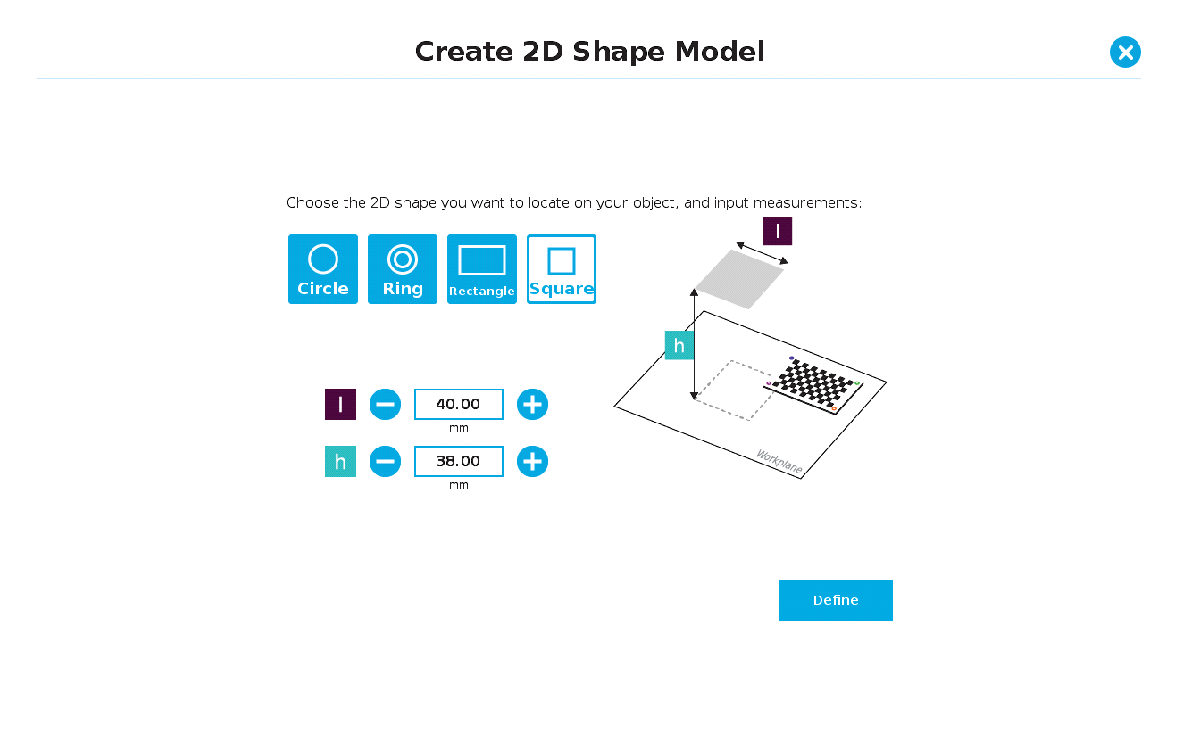
\includegraphics[width=0.7\textwidth]{ur5e_cam_param.eps}
%\caption{Nastavitve parametrov objekta}
%\label{fig:ur_cam_param}
%\end{figure}
%
%V naslednjem koraku vam program že prepozna objekt, če se le-ta nahaja v vidnem polju kamere. če izberete prepoznan objekt, lahko s klikom na ikono koordinatnega sistema levo zgoraj dobite informacije o prepoznani legi objekta. Z izbiro ikone s kockami (leva stran, druga od zgoraj dol) lahko nastavite število prepoznanih objektov, če je le-to več od ena.
%
%\begin{figure}[!hbt]
%\centering
%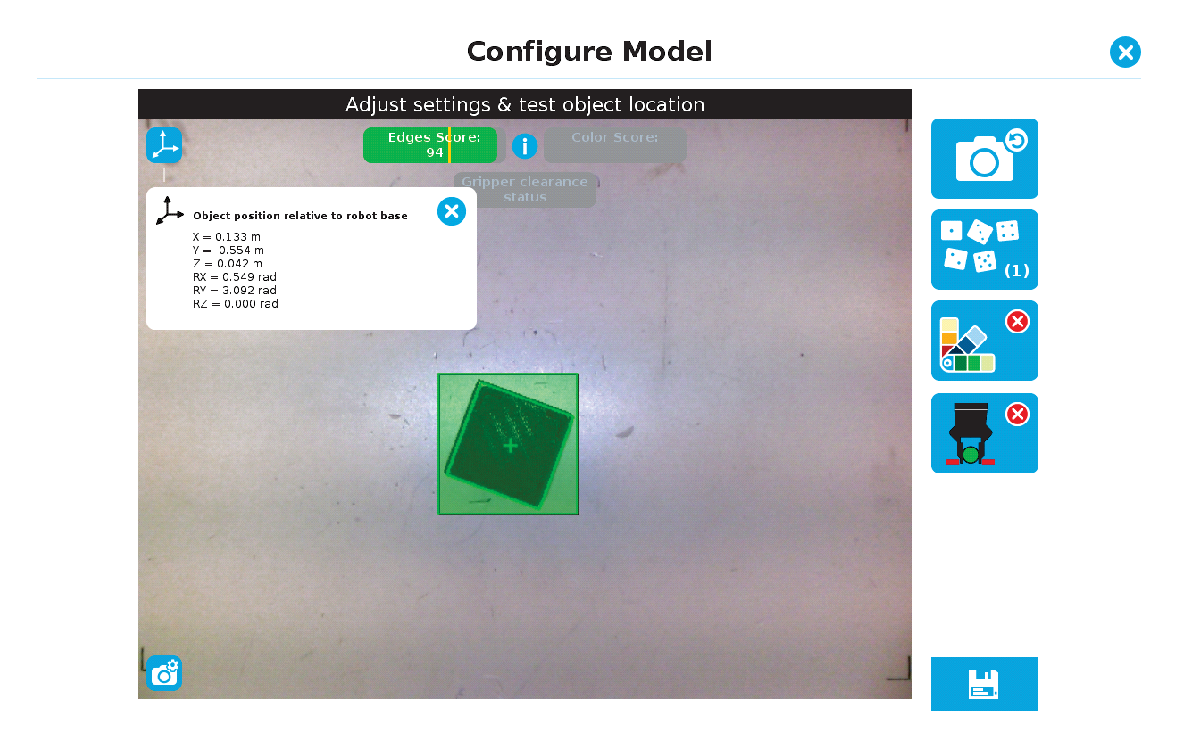
\includegraphics[width=0.7\textwidth]{ur5e_cam_objekt.eps}
%\caption{Prepoznan objekt}
%\label{fig:ur_cam_objekt}
%\end{figure}
%
%
%
%\subsection{Program}
%
%
%V programu je potrebno pred ukaz \verb"Camera Locate" dodati ukaz \verb"MoveJ", kjer premaknete robota v lego za slikanje (\emph{Snapshot position}).
%
%Nato postavite v vidno polje kamere en objekt, v ukazu \verb"Camera Locate" pa izberete \emph{Test/Modify}. Odpre se vam okno z živo sliko kamere. Ob kliku na ikono fotoaparata (leva stran, prva ikona) kamera zajeme novo sliko,  program pa izvede prepoznavo objekta. Za potrditev prepoznane lege kliknite na ikono diskete desno spodaj. Na ta način shranite trenutno lego prepoznanega objekta pod ukaz \verb"Camera Locate".
%
%Ukaz \verb"Camera Locate" deluje kot pogojni  \verb"If" stavek. če je naučen objekt prepoznan, potem bo robotski program izvršil kodo znotraj pogojnega stavka.
%
%Ko zaključite z uporabo čarovnika za učenje objektov, se shrani zadnja lega prepoznanega objekta (pozicija v smer $x$ in $y$ ter kot okoli osi $z$). Spremenljivka, ki vsebuje lego objekta, je poimenovana po \emph{Snapshot position} in vsebuje informacijo o legi koordinatnega sistema prepoznanega objekta glede na shranjeno lego robota. Vsako iteracijo, ko kamera prepozna objekt in se izvede \verb"Camera Locate", se posodobi ta spremenljivka z lego na novo prepoznanega objekta. Koordinatni sistem, ki nosi to informacijo, je poimenovan enako kot je bila poimenovan \emph{Snapshot Position}.
%
%V nadaljevanju je potrebno napisati program za manipulacijo objektov.  Premiki za prijem objekta morajo biti definirani relativno glede na koordinatni sistem lege kamera (pri ukazu \emph{Move} v zavihku \emph{Command} definirate \emph{Feature} kot ustrezen \emph{Snapshot position}).
%
%Ker ste že slikali en objekt, imate informacijo o legi objekta na voljo. Osnovna manipulacija zajema štiri korake
%\begin{itemize}
%    \item premik robota nad objekt (gib \verb"MoveJ");
%    \item premik robota do objekta (gib \verb"MoveL");
%    \item zapiranje prijemala;
%    \item dvig objekta z robotom (gib \verb"MoveL").
%\end{itemize}
%
%\begin{mdframed}[backgroundcolor=yellow!20, shadow=true,roundcorner=8pt]
%\textbf{OPOZORILO:} Med postopkom učenja manipulacije z objekti (prva in druga točka zgoraj) ne premikajte objektov!
%\end{mdframed}
%
%Primer implementacije programa je podan v nadaljevanju.
%
%\begin{verbatim}
%Robot Program
%  Camera Locate
%    For object(s) found
%      MoveJ
%        nadObjekt
%      MoveL
%        doObjekta
%        Gripper Close(2)
%        nadObjekt
%\end{verbatim}


\section{Tekoči trak}

Ključni elementi tekočega traku so, poleg transportnega traku, relativni inkrementalni dajalnik pozicije ter laserski senzor, ki prepozna, kdaj objekt prečka določeno točko na traku.

Ko objekt prekine laserski žarek, robot začne slediti objektu. Število pulzov inkrementalnega dajalnika nam pove, kolikšno razdaljo je prepotoval objekt. Razdalja $d$ je podana kot
\begin{equation}\
  d = \frac{n}{CPM} \, ,
\end{equation}
pri čemer je $n$ število izmerjenih pulzov, $CPM$ pa število pulzov, ki jih vrne inkrementalni dajalnik, ko tekoči trak prepotuje razdaljo 1~m (v našem primeru je $CPM = 8700$~pulzov/m). Smer tekočega traku je določena s koordinatnim sistemom tekočega traku, ki je definiran v \emph{Features} kot linija \emph{tekoci\_trak}.

\section{Naloga}

% a) kalibracija orodja
% b) tekoci trak
% - definiranje tocke pristopa
% - definiranje tocke prijemanja
% c) vstavljanje zobnika na os
% - poisci os - insertion/spiral
% - poisci kajlo - insertion/rotational



Naloga zajema vstavljanje zobnika na os z zagozdo. Najprej bo robot sledil zobniku na tekočem traku ter ga pobral. Nato boste s spiralnim gibom na podlagi izmerjene sile poiskali os, pri vstavljanju zobnika pa uporabili še rotacijo, da bo robot avtomatsko detektiral zagozdo na os.

\subsection{Naloga 1: Kalibracija prijemala}


Najprej pripravite nov program, tako da v zgornji orodni vrstici izberete \emph{New... >  Program}.
\begin{itemize}
  \item Vklopite sekvenco programa, ki služi kot inicializacija: \emph{Robot Program > Add Before Start Sequence}.
  \item Izklopite ponavljanje programa: \emph{Robot Program > Program Loops Forever} -- odkljukate.
\end{itemize}
Nato naložite še ustrezno datoteko z nastavitvami (\emph{.installation}).
\begin{itemize}
    \item V zgornji vrtici izberete \emph{Open... > Installation}.
    \item Premaknite se v mapo \verb"OR\tmpInstallation" ter označite datoteko \verb"orINST.installation", ki jo naložite z izbiro gumba \emph{Open}.
    \item Na vprašanje, če želite posodobiti program, odgovorite pritrdilno (\emph{Update Program}).
    \item Naložene nastavitve shranite z novim imenom: \emph{Save... > Save Installation As...}, kjer ponovno izberete mapo \verb"OR", nastavite \textbf{novo ime} datoteke z nastavitvami ter izberete \emph{Save}.
    \item Ponovno zaženete robota (poglavje \ref{ch:zagon}).
\end{itemize}

V datoteki \verb"orINST.installation" se nahajajo nastavitve tekočega traku.

V nadaljevanju definirajte parametre orodja:
\begin{itemize}
  \item TCP -- vrh orodja;
  \item Payload -- skupna masa orodja in obdelovanca;
  \item COG -- težišče.
\end{itemize}

\begin{mdframed}[backgroundcolor=blue!20, shadow=true,roundcorner=8pt]
\textbf{INFO:} Robot za svoje delovanje in izvajanje varnostnih funkcij uporablja dinamični model, zato je pomembno, da so parametri orodja nastavljeni pravilno. Kot primer: če je vpisana teža prijemala prevelika, bo robot kompenziral težo prijemala s prevelikimi navori v sklepih. Kot rezultat, se bo robot nepričakovano premaknil navzgor.
\end{mdframed}


TCP se nastavi v zavihu \emph{Installation}, razdelek \emph{Setup for the Tool Center Point}, kot je prikazano na sliki \ref{fig:ur_install}. Vsaka definicija TCP zajema translacijo in rotacijo do vrha orodja relativno na središče vrha robota. Točke v programu so shranjene glede na lego TCP, zato je pomembno, da je izbrano pravilno orodje tako za učenje točk kot tudi za izvajanje programa.

\begin{figure}[!hbt]
\centering
 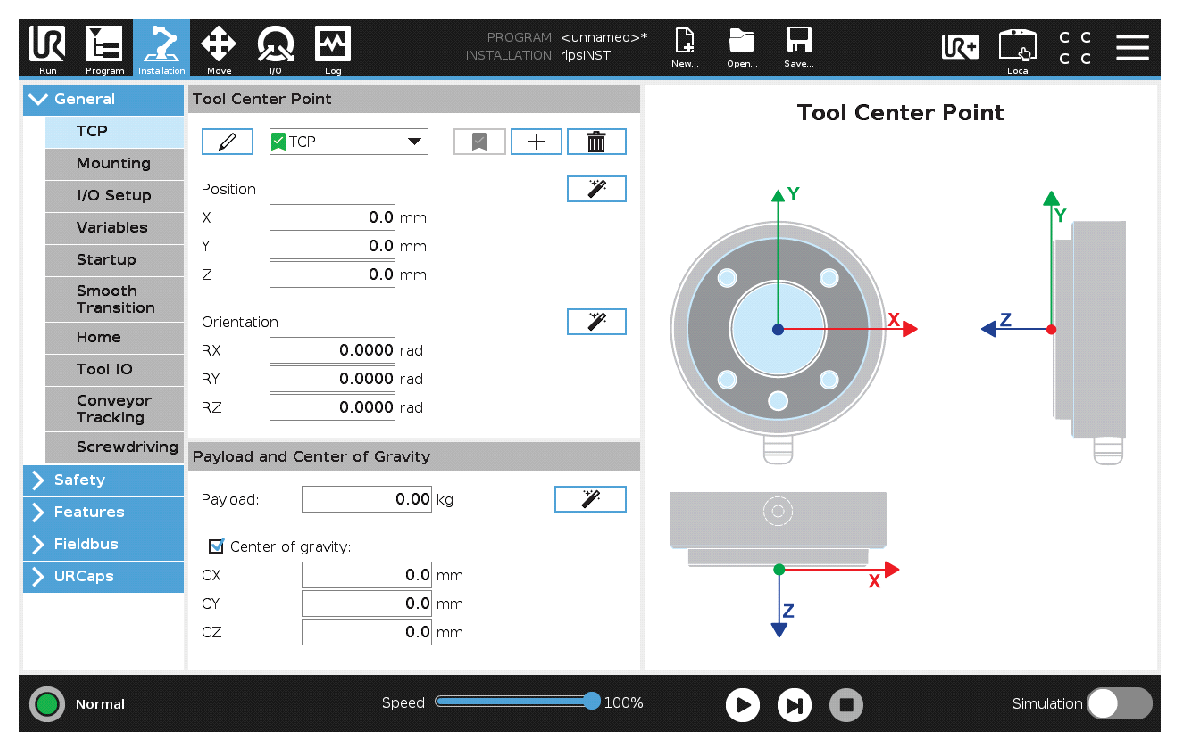
\includegraphics[width=0.7\textwidth]{ur5e_tcp.eps}
\caption{Okno za nastavljanje parametrov orodja}
\label{fig:ur_install}
\end{figure}


Vrednosti \emph{X}, \emph{Y} in \emph{Z} opisujejo pozicijo orodja, medtem ko \emph{RX}, \emph{RY} in \emph{RZ} opisujejo njegovo rotacijo. Če so vse vrednosti nastavljene na 0, potem koordinatni sistem orodja sovpada s koordinatnim sistemom vrha robota.


\begin{mdframed}[backgroundcolor=yellow!20, shadow=true,roundcorner=8pt]
V bela polja poleg posameznih spremenljivk vpišite ustrezne vrednosti, da definirate prijemalo, kot je podano na sliki \ref{fig:ur_gripper}. Pri tem upoštevajte še debelino kamere, ki znaša 13,5~mm.
\end{mdframed}


Maso in težišče robota se definira v spodnjem delu zaslona. Ponovno se lahko vpiše posamezne vrednosti v bela polja, ali pa se uporabi čarovnik za določevanje parametrov.

\begin{mdframed}[backgroundcolor=yellow!20, shadow=true,roundcorner=8pt]
Uporabite čarovnik za oceno mase in težišča prijemala.
\end{mdframed}

Čarovnik zahteva sledeči postopek:
\begin{enumerate}
\item v zavihku \emph{Installation} pod \emph{General} izberite \emph{TCP};
\item v predelku \emph{Payload and Center of Gravity} izberite \emph{Payload and Center of Gravity Wizard} -- ikona čarobne palice;
\item v čarovniku izberite \emph{Next};
\item sledite navodilom na ekranu; premaknite in shranite štiri različne lege robota;
\item ko shranite vse štiri lege, izberite \emph{Finish}.
\end{enumerate}

Končna deklaracija prijemala mora biti podobna kot v tabeli \ref{tab:tcp}.

\begin{center}
\begin{tabular}{|l|c|}
  \hline
  % after \\: \hline or \cline{col1-col2} \cline{col3-col4} ...
  TCP & [$0$, $0$, $159,5$]~mm \\
  \hline
  Payload & $1,135$ kg \\
  \hline
  COG & [$-0,6$, $1,0$, $57,4$]~mm\\
  \hline
\end{tabular}
\label{tab:tcp}
\end{center}

\begin{mdframed}[backgroundcolor=blue!20, shadow=true,roundcorner=8pt]
\textbf{OPOMBA:} Štiri TCP lege naj bodo čimbolj različne.
\end{mdframed}

Robota sedaj postavite v začetno lego.  V meniju \emph{Move} nastavite kote v sklepih na

\begin{tabular}{|r|c|}
  \hline
  % after \\: \hline or \cline{col1-col2} \cline{col3-col4} ...
  Base & $0^\circ$ \\
  Shoulder & $-90^\circ$ \\
  Elbow & $-90^\circ$ \\
  Wrist 1 & $-90^\circ$ \\
  Wrist 2 & $90^\circ$ \\
  Wrist 3 & 0 \\
  \hline
\end{tabular}

nato pa izberete \emph{OK} in držite \emph{Move robot to: New position}.

%\begin{mdframed}[backgroundcolor=yellow!20, shadow=true,roundcorner=8pt]
%\textbf{OPOZORILO:} Izogibajte se prijemanju/vlečenju/porivanju orodja pred in med izvajanjem estimacije.
%\end{mdframed}


\subsection{Naloga 2: Manipulacija objekta na tekočem traku}

V naslednjem delu boste napisali program za manipulacijo enega objekta na tekočem traku. Pri tem sledite navodilom v nadaljevanju.

\begin{mdframed}[backgroundcolor=yellow!20, shadow=true,roundcorner=8pt]
\begin{itemize}
  \item Pod \verb"BeforeStart" dodajte ukaz za aktivacijo prijemala
  \item Pod \verb"Robot Program" dodajte ukaz za odprtje prijemala (\emph{URCaps > Gripper > Edit Action > Open > Save Action}).
  \item Postavite robota v poljubno začetno lego (slika \ref{fig:ur_lega1} levo) in shranite gib kot \verb"MoveJ". Višina robota naj bo nad višino tekočega traku, prijemalo pa naj bo orientirano vzdolž osi z. Pri ukazu \verb"MoveJ" mora biti pod \emph{Feature} izbran \emph{Base}. Ukaz za premik shranite po sledečem postopku:
      \begin{itemize}
        \item dodajte ukaz \emph{Basic > Move};
        \item v zavihku \emph{Command} izberite ustrezen tip giba;
        \item kliknite na \emph{Waypoint} pod ukazom \emph{Move} (obarvano rumeno) in izberite \emph{Set Waypoint > OK}, da shranite lego robota;
        \item če želite dodati novo točko pod isti gibom, lahko dodate nov \emph{Basic > Waypoint}.
      \end{itemize}
  \item Na tekoči trak postavite zobnik na mesto, kjer zobnik ravno prekine laserski žarek.
    \item  V zavihku \emph{I/O} lahko preverite, če je digitalni vhod 1 (laser) postavljen na visok nivo.
  \item Premaknite robota nad tekoči trak na mesto, kjer bo čakal na zobnik (slika \ref{fig:ur_lega1} desno). Gib shranite kot \verb"MoveJ".
%\end{itemize}
%\end{mdframed}
%
%
%
%\begin{mdframed}[backgroundcolor=yellow!20, shadow=true,roundcorner=8pt]
%\begin{itemize}
  \item Vstavite ukaz za vklop tekočega traku: \emph{Basic > Set > Set Digital Output: tekociTrak: High}.
  \item Nato naj program čaka, da predmet prekine laserski žarek \emph{Basic > Wait > Wait for Digital Input: laser: High}.
  \item V program dodajte predlogo za tekoči trak:  \emph{Templates > Conveyor Tracking}. Izberite \emph{Conveyor 1}. Naslednji ukazi morajo biti ugnezdeni pod \verb"Tracking Conveyor".
  \begin{itemize}
      \item Dodajte še ukaz \emph{Wait}, da robot počaka 2 sekundi, preden pobere objekt.
      \item Sedaj morate robota naučiti še dve legi:
      \begin{itemize}
        \item lego nad objektom, v kateri bo robot sledil objektu (robot je postavljen nad zobnik, slika \ref{fig:ur_ucenje_TT} zgoraj);
        \item lego prijemanja objekta, kjer premaknete robota do vrha zobnika (slika \ref{fig:ur_ucenje_TT} spodaj).
      \end{itemize}
      Ti dve legi naučite, ko je objekt na tekočem traku v poziciji, ko ravno prekine laserski žarek (takrat začne robot slediti objektu). Pri tem uporabite linearni gib s hitrostjo 100~mm/s.
      \item Dodajte še ukaz za zaprtje prijemala (nastavitve \emph{Position}: 85~\%, \emph{Speed}: 50~\%, \emph{Force}: 30~\%).
  \end{itemize}
  \item Robota naučite še eno točko nad tekočim trakom (slika \ref{fig:ur_after}), kamor se bo robot premaknil, ko bo prijel objekt (linearni gib). Ta ukaz mora biti ugnezden pod \verb"Robot Program" ne več pod \verb"Tracking" \verb"Conveyor".
  \item Dodajte še ukaz za ustavitev tekočega traku: \emph{Basic > Set > Set Digital Output: tekociTrak: Low}.
 \end{itemize}
\end{mdframed}

   \begin{figure}[!htb]
\centering
 \includegraphics[width=0.8\textwidth]{ur5e_lega1.eps}
\caption{Primer začetne lege (levo) in lege, v kateri robot čaka na zobnik (desno)}
\label{fig:ur_lega1}
\end{figure}

   \begin{figure}[!htb]
\centering
 \includegraphics[width=0.8\textwidth]{ur5e_ucenje_TT.eps}
\caption{Lega za sledenje objektu (zgoraj) in lega za prijemanje objekta (spodaj)}
\label{fig:ur_ucenje_TT}
\end{figure}



  \begin{mdframed}[backgroundcolor=yellow!20, shadow=true,roundcorner=8pt]
\begin{itemize}
    \item Zobnik postavi na začetek tekočega traku.
  \item Testirajte vaš program: gumb \emph{Play > Move Robot To:} (gumb držite pritisnjen) \emph{> Play from: Robot Program}.
\end{itemize}
\end{mdframed}



  \begin{figure}[!hbt]
\centering
 \includegraphics[width=0.4\textwidth]{ur5e_po_prijetju.eps}
\caption{Primer lege, v katero se premakne robot, po tem ko prime objekt}
\label{fig:ur_after}
\end{figure}


\subsection{Naloga 3: Vstavljanje zobnika na os}

Vstavljanje zobnika na os poteka na podlagi senzorja sile v treh fazah:
\begin{enumerate}
  \item poiščete os s spiralnim gibanjem (funkcija \emph{Insertion > Spiral});
  \item z vrtenjem okoli osi poiščete zagozdo (funkcija \emph{Insertion > Rotational});
  \item zobnik potisnite do konca osi (funkcija \emph{Insertion > Linear}).
\end{enumerate}


\begin{mdframed}[backgroundcolor=yellow!20, shadow=true,roundcorner=8pt]
\begin{itemize}
  \item Premaknite robota 10~cm nad os; gib shranite kot \verb"MoveJ".
  \item Zobnik premaknite približno nad os; pomagajte si z različnimi pogledi kamere. Gib shranite kot \verb"MoveL". Primer postavitve je predstavljen na sliki \ref{fig:ur_nad_osjo}.
\end{itemize}
\end{mdframed}
  \begin{figure}[!hbt]
\centering
 \includegraphics[width=0.8\textwidth]{ur5e_nad_osjo.eps}
\caption{Zobnik, postavljen nad os. Ta lega predstavlja začetno lego, v kateri bo robot začel z iskanjem osi.}
\label{fig:ur_nad_osjo}
\end{figure}

  \begin{mdframed}[backgroundcolor=yellow!20, shadow=true,roundcorner=8pt]
\begin{itemize}
  \item Dodajte ukaz za spiralno gibanje za iskanje osi: \emph{URCaps > Insertion > Spiral}.
  \item Ko kliknete na \verb"Spiral", lahko nastavljate parametre kot so
  \begin{itemize}
        \item A -- ciljna točka;
        \item B -- smer giba;
        \item C -- hitrost premikanja;
        \item D -- sila, pri kateri se inicializira gib;
        \item E -- korak radija;
        \item F -- največji radij;
        \item G -- sila, pri kateri se začne vstavljanje.
  \end{itemize}
  Pri tem gibu je pomembna samo višina, do katere mora robot potisniti zobnik, zato ni pomembno, če je zobnik na osi ali poleg nje. Začetno točko določa prejšnja točka, za fino poravnavo pa poskrbi sama funkcija. Zobnik z robotom premaknite med os in tekoči trak, nato pa ga spustite na tako višino, da je spodnji rob zobnika malo nad zagozdo (slika \ref{fig:ur_visina} levo).
  To točko shranite kot \emph{Destination (A)} z gumbom \emph{Teach position}. Smer gibanja \emph{Direction (B)} mora biti nastavljena na \verb"Z+". če robota z zobnikom vrnete v točko nad osjo (v programu izberete točko in držite pritisnjen gumb \emph{Move here}), lahko testirate delovanje z gumbom \emph{Hold to test}.
  \item Po končanem testu premaknite robota navzgor po \verb"Z+" osi, da preprečite trk med robotom in osjo.
  \end{itemize}
\end{mdframed}

\begin{figure}[!hbt]
\centering
 \includegraphics[width=0.8\textwidth]{ur5e_visina.eps}
\caption{Višina zobnika pri iskanju osi (levo, ukaz \emph{Spiral}) in višina zobnika pri iskanju zagozde (desno, ukaz \emph{Rotational})}
\label{fig:ur_visina}
\end{figure}


    \begin{mdframed}[backgroundcolor=yellow!20, shadow=true,roundcorner=8pt]
\begin{itemize}
  \item Dodajte še ukaz za detekcijo zagozde. V programu kliknete na \verb"Insertion" in izberete \emph{Rotational}.
  \item Ko kliknete na \verb"Rotational", lahko nastavite parametre kot so
   \begin{itemize}
          \item A -- ciljna točka;
          \item B -- smer premika;
          \item C -- linearna hitrost;
          \item D -- sila, potrebna za začetek rotacije;
          \item E -- največji kot rotacije.
  \end{itemize}
  Podobno kot pri spiralnem gibu je tudi tu pomembna samo globina premika. Za začetno točko poskrbi spiralni gib, za ostalo pa sama funkcija. Z robotom se ponovno postavite med os in tekoči trak, spodnji rob zobnika pa premaknite skoraj do konca osi (slika \ref{fig:ur_visina} desno). To točko shranite kot \emph{Destination (A)} z gumbom \emph{Teach position}. Smer gibanja \emph{Direction (B)} mora biti nastavljena na \verb"Z+". Ponovno lahko testirate delovanje, tako da se postavite v točko nad osjo, testirate \verb"Spiral" in nato še \verb"Rotational".
  \item Da potisnete zobnik do konca osi boste uporabili funkcijo \emph{Linear} (\verb"Insertion" \emph{Linear}). Pri tej funkciji se robot premika v določeni smeri, dokler ne zazna nastavljene sile. Robot naj se premika v \emph{Z$+$} smeri v koordinatnem sistemu orodja. Mejno sile nastavite na 20~N (\emph{Advanced Parameters > Force threshold (C)}).
  \item Dodajte še ukaz za odprtje prijemala: \emph{URCaps > Gripper > Edit action > Open}.
  \item Premaknite robota nad zobnik -- linearni gib.
  \item Premaknite robota v začetno lego -- \emph{MoveJ}.
  \item Zobnik postavite na začetek tekočega traku.
   \item Testirajte vaš program: gumb \emph{Play > Move Robot To: > Play from: Robot Program}.
  \end{itemize}
\end{mdframed}


